\chapter{The Sphere Packing Problem in Dimension $8$}
\thispagestyle{empty}
% It might be worth chucking a large part of this chapter into an appendix. Specifically, §2.1.1 (Sphere Packing Fundamentals) and §2.3 (Modular Forms). Need to think about this... this would also depend on how we phrase §1.3 (scope of project) because we need to make it EXTREMELY CLEAR that the purpose of this project was NOT to delve deep into a cool application of the theory of modular forms but rather to learn how to formalise modern, computationally involved mathematics.

The purpose of this chapter is to conduct a detailed examination of Viazovska's original paper solving the sphere packing problem in dimension $8$ \cite{Viazovska8} and the formalisation blueprint \cite{blueprint}. While we have already seen the high-level idea in \Cref{Ch1:Sec:1_1_Sphere_Packing}, in this chapter, we will take a closer look at the mathematical details.

We will begin by providing precise mathematical definitions for sphere packings, densities, and the sphere packing constant. We will then discuss the linear programming bound conceived by Cohn and Elkies \cite[Theorem 3.1]{CohnElkies} (or, more precisely, the slight modification thereof that is more directly applicable: see \cite[Theorem 2]{Viazovska8} and \cite[Theorem 5.1]{blueprint}). Finally, we will include a small discussion on the theory of modular forms and establish its relevance to the subsequent chapters of this thesis, which will focus on the construction of the `Magic Function' (denoted as $g$ in \cite[Theorem 3]{Viazovska8}).

In each section, we will not only mathematical details from the sources outlined above but also an overview of the choices made and challenges encountered when formalising these notions. While this chapter primarily concerns the contents of the first three sections of \cite{Viazovska8}, which are not within the scope of this project, there is an undeniable relevance of both the informal and the formal definitions and results. It is therefore necessary to include a detailed treatment thereof before we can construct $g$ and prove it satisfies the desired `Magic' properties.

\section{Preliminaries}

Before we begin defining things formally, we must include a small disclaimer about the terminology we have been using---and will continue to use---in this project. While \Cref{Ch1:Prob:SpherePacking_n} is usually referred to as the \textit{sphere} packing problem, a sphere is not usually thought to have an interior. Typically, in any metric space $X$ with metric $d$, the \textit{sphere} of radius $r \geq 0$ centred at $x \in X$ is defined to be $\setst{y \in X}{d(x, y) = r}$. In other words, the sphere consists only of a surface. In contrast, the sphere packing problem involves packing \textit{solid balls}. One can see why, in \cite{CannonHoney}, Hales opines that a more proper term for the problem would be the \textit{ball packing problem}. Nevertheless, in this project, we will continue to use the standard terminology, but we include this disclaimer so the reader bears in mind two things: first, that we will often mean `ball' when we use the word `sphere', and second, that we work with balls instead of spheres in Lean. We will also mention that it is convenient to require that the balls in question be open, so that the condition that spheres cannot overlap but merely touch tangentially can be shortened to that of disjointedness. We introduce notation.

\begin{boxnotation}
    For some $d \in \N$, $x \in \R^d$ and $r > 0$, we denote
    \begin{align*}
        B_d(x, r) := \setst{y \in \R^d}{\norm{x - y} < r}
    \end{align*}
\end{boxnotation}

We organise this section into three subsections. The first defines fundamental notions about sphere packings. The second introduces the properties of two important, and closely related, classes of sphere packings, namely, lattice packings and periodic packings. The third subsection studies the most important sphere packing for our project: the $E_8$ lattice packing.

\subsection{Sphere Packing Fundamentals}

We begin by defining a sphere packing. As we have stated, we want sphere packings to consist of disjoint spheres of the same radius. Given that lying on the interior of a certain sphere corresponds to being within some distance from its centre, we can capture this notion of disjointedness by imposing a separation condition on the set of centres of the sphere packing.

\begin{boxdefinition}[Sphere Packing]
    Fix $d \in \N$ and $X \subset \R^d$. Assume that there exists a real number $r > 0$, known as the \textbf{separation radius}, such that
    \begin{align*}
        \norm{x - y} \geq r
    \end{align*}
    for all distinct $x, y \in X$. We define the \textbf{sphere packing with centres at $X$} to be
    \begin{align*}
        \Pa(X) := \bigcup_{x \in X} B_d(x, r)
    \end{align*}
\end{boxdefinition}

Note that the assumption that a separation radius exists is very important.

\begin{boxnexample}
    Let $d = 1$ and $X = \R$. Consider the set
    \begin{align*}
        \bigcup_{x \in \R} B_1(x, r) = \bigcup_{x \in \R} \parenth{x-r, x+r}
    \end{align*}
    For any $r > 0$, the above union is all of $\R$. However, it does not make sense to construct a sphere packing whose set of centres is the entirety of $\R$, as this would involve spheres overlapping. It is precisely to avoid such constructions that we impose the condition that $r$ be a separation radius on the set of centres.
\end{boxnexample}

Since all the information about a sphere packing is encoded in its set of centres and the corresponding separation radius (which must exist in order for the set of centres to be a valid set of centres for a sphere packing), we decided that a sphere packing would be formalised purely as a set of centres with a valid separation, and that a separate definition would be made to obtain the open balls that constitute the packing. We packaged the data of
\begin{itemize}
    \item the set of centres
    \item the separation radius
    \item the (automatically checked) condition that the separation radius is positive
    \item the condition that the set of centres is, indeed, separated by this radius
\end{itemize}
into a \verb|structure| called \verb|SpherePacking|: see \cite[\texttt{SpherePacking.Basic.SpherePacking}]{documentation}.\todo{Is this an acceptable way of citing the documentation? Should the repo be made public?}

We now define finite density, an indicator of how much of a bounded region of space a sphere packing covers.

\begin{boxdefinition}[Finite Density]\label{Ch2:Def:FiniteDensity}
    Let $\Pa$ be a sphere packing. For all $R > 0$, define the \textbf{finite density} to be
    \begin{align*}
        \Delta_\Pa(R) := \frac{\Volof{\Pa \cap B_d(0, R)}}{\Volof{B_d(0, R)}}
    \end{align*}
    where $\Vol$ is the Lebesgue measure on $\R^d$.
\end{boxdefinition}

Finite density is a somewhat local notion, in that it expresses sphere how closely packed spheres are in a bounded region. The sphere packing problem, on the other hand, examines the notion of closeness on a more global level. While taking the limit of finite densities as the radius of the bounding region approaches infinity might seem like a natural way to define density, it is not obvious that this limit always exists. Therefore, we define density to be the limit superior instead.

\begin{boxdefinition}[Density]\label{Ch2:Def:Density}
    Let $\Pa$ be a sphere packing. Define the \textbf{density} of $\Pa$ to be
    \begin{align*}
        \Delta(\Pa) := \limsup_{R \to \infty} \Delta_\Pa(R)
    \end{align*}
    where $\Delta_\Pa(R)$ is the finite density of $\Pa$, as defined in \Cref{Ch2:Def:FiniteDensity}.
\end{boxdefinition}

As one might expect, finite density and density are invariant under scaling.

\begin{boxproposition}\label{Ch2:Prop:Scaling_Sphere_Packings}
    Let $\Pa$ be a sphere packing. Fix $\lambda > 0$. Denoting by $\lambda \Pa$ the sphere packing obtained by scaling the spheres and the set of centres in $\Pa$ by a factor of $\lambda$, we have
    \begin{align*}
        \Delta_{\Pa}\of{R} = \Delta_{\lambda \Pa}\of{\lambda R}
    \end{align*}
    for all $R > 0$. Similarly, we have
    \begin{align*}
        \Delta\of{\Pa} = \Delta\of{\lambda \Pa}
    \end{align*}
\end{boxproposition}

The sphere packing problem asks for the sphere packing that achieves the highest possible density. We can be formal about the notion of the highest possible density.

\begin{boxdefinition}[Sphere Packing Constant]
    The \textbf{sphere packing constant} in $\R^d$, for any $d > 0$, is defined to be
    \begin{align*}
        \Delta_d := \sup\!\parenth{{\setst{\Delta_{\Pa}}{\Pa \text{ is a sphere packing in } \R^d}}}
    \end{align*}
\end{boxdefinition}

\Cref{Ch2:Prop:Scaling_Sphere_Packings} tells us that it suffices to take the supremum over sphere packings of separation $1$, because a sphere packing $\Pa$ can be scaled down by its separation radius to obtain a sphere packing of separation $1$.

\begin{boxproposition}\label{Ch2:Prop:Scaling_Sphere_Packing_Constant}
    For all $d$, we have
    \begin{align*}
        \Delta_d = \sup\!\parenth{{\setst{\Delta_{\Pa}}{\Pa \text{ is a sphere packing in } \R^d \text{ with separation } 1}}}
    \end{align*}
\end{boxproposition}

As intuitive as this result might seem, we do mention it here because it is something we have to deal with explicitly when formalising the theory of sphere packings in Lean. The first instance when we really see it in action is the proof of \Cref{SP:Thm:CohnElkies}.

The objective of the sphere packing problem in any dimension $d$ is to optimise the sphere packing constant $\Delta_d$. As we have seen, this is a highly non-trivial thing to do. We can, however, offer a trivial upper-bound on sphere packing density.

\begin{boxlemma}
    For any sphere packing $\Pa$ and $R > 0$, we have that $\Delta_{\Pa}(R) \leq 1$.
\end{boxlemma}
\begin{proof}
    This is an immediate consequence of the fact that $\Pa \cap B_d(0, R) \subseteq B_d(0, R)$.
\end{proof}
This immediately gives us the following basic facts.
\begin{boxcorollary}
    For any sphere packing $\Pa$, we have that $\Delta_{\Pa} \leq 1$.
\end{boxcorollary}
\begin{boxcorollary}
    For any $d \in \N$, $\Delta_d \leq 1$.
\end{boxcorollary}

This is not a very good upper-bound. However, it tells us that the sphere packing constant in any number of dimensions is a finite real number in the interval $(0, 1]$. There is still some work to be done before we can give better bounds on the sphere packing constant. Furthermore, it is unclear whether the sphere packing constant actually is, for a general $d$, the density of a sphere packing in $\R^d$. Nevertheless, this is a good starting point.

A great deal of basic sphere packing API in Lean was developed in July 2024 for the project to formalise Viazovska's solution in dimensino $8$. The majority of the code was written by Gareth Ma, who also made significant improvements to the design choices I had made when setting up the project. The definitions and results in this section have all been formalised, and information about the code that has been written can be found in the project documentation \cite[\texttt{SpherePacking.Basic.SpherePacking}]{documentation}.

In the next subsection, we discuss a special class of sphere packings that have periodicity properties with respect to lattices.

\subsection{Lattice and Periodic Sphere Packings}

We begin by defining lattices and briefly commenting on existing \verb|Mathlib| API on lattices. There are primarily two ways in which lattices are defined in mathematical literature. A lattice in some Euclidean space $\R^n$ is either described as the $\Z$-span of some $\R$-basis of $\R^n$ or as a discrete, co-compact subgroup. One can borrow characteristics from both definitions to construct other equivalent definitions.

The characteristics described in both definitions do exist \verb|Mathlib|. However, given that one of the objectives of creating a unified mathematics library is centralisation, a combination of these definitions is used as the \textit{definition} of a \verb|class| that we call \verb|IsZLattice| and information about its many properties, as well as the $\Z$-span construction, are encoded in theorems. In particular, we have a theorem that tell us that every lattice is a free $\Z$-submodule, meaning it has a $\Z$-basis, and that this $\Z$-basis is actually an $\R$-basis of the ambient space. Furthermore, we have a result that every object constructed in that manner is a lattice. Results about types bearing the \verb|IsZLattice| class (ie, lattices as they are defined in \verb|Mathlib|) live in the \verb|ZLattice| namespace, whereas results bout $\Z$-spans of $\R$-bases live in the \verb|ZSpan| namespace. \todo{Create citation for Mathlib.}

We begin by stating the \verb|Mathlib| definition of a lattice.

\begin{boxdefinition}[Lattice]
    A \textbf{lattice} in a Euclidean space $\R^n$ is a discrete $\Z$-submodule of $\R^n$ such that its $\R$-span contains every element in $\R^n$.
\end{boxdefinition}

The \verb|Mathlib| definition is more general, and works for any normed vector space over a normed field. Here, the word `discrete' means that the lattice is discrete in a topological sense, meaning that the subspace topology on the lattice is precisely the discrete topology.

\begin{boxdefinition}[Periodic Sphere Packing]
    Let $\Lambda \subset \R^d$ be a lattice. We say a sphere packing $\Pa(X)$ with spheres centred at points in $X \subset \R^d$ is \textbf{periodic with respect to $\Lambda$}, or \textbf{$\Lambda$-periodic},
    \begin{align*}
        \lambda + X = X
    \end{align*}
    ie, for all $\lambda \in \Lambda$ and $x \in X$, we have that $\lambda + x \in X$.
\end{boxdefinition}

We define Periodic Sphere Packings in Lean as extending the definition of Sphere Packings by creating a \verb|structure| called \verb|PeriodicSpherePacking| that packages the additional data of
\begin{itemize}
    \item the lattice, viewed as a $\Z$-submodule of the ambient space $\R^d$
    \item the condition that the set of centres is periodic with respect to this $\Z$-submodule
    \item the (automatically checked) condition\footnotemark{} that the $\Z$-submodule is discrete
    \item the (automatically checked) condition\footnotemark[\value{footnote}] that the discrete $\Z$-submodule is a lattice
\end{itemize}
\footnotetext{more precisely, the automatically inferred instance}
The definition is in \cite[\texttt{SpherePacking.Basic.SpherePacking}]{documentation}.

Lattice packings are a special class of periodic packings.

\begin{boxdefinition}[Lattice Packing]
    Let $\Lambda \subset \R^d$ be a lattice. The \textbf{$\Lambda$ lattice packing} is the sphere packing with centres at points in $\Lambda$. Such a sphere packing admits a separation radius because $\Lambda$ is discrete and is $\Lambda$-periodic because $\Lambda$ is closed under addition.
\end{boxdefinition}

In \Cref{Ch2:Subsec:E8}, we will briefly examine a specific lattice packing, the $E_8$ lattice packing.

The periodicity property of a periodic sphere packing can be exploited to derive a more convenient formula for its density.

\begin{boxproposition}\label{Ch2:Prop:Periodic_Density}
    Let $\Pa(X)$ be a sphere packing with centres at $X \subset \R^d$ and separation $r$ that is periodic with respect to some lattice $\Lambda \subset \R^d$. We have that
    \begin{align}
        \Delta_{\Pa(X)} = \abs{\quotient{X}{\Lambda}} \frac{\Volof{B_d\of{0, \frac{r}{2}}}}{\Volof{\quotient{\R^d}{\Lambda}}}
        \label{Ch2:Eq:Periodic_Density}
    \end{align}
    where $\abs{\quotient{X}{\Lambda}}$ is the number of orbits of the additive $\Lambda$-action on $X$ and $\Volof{\quotient{\R^d}{\Lambda}}$ is the volume of the fundamental domain of the $\Lambda$-action on $\R^d$.
\end{boxproposition}

The proof is beyond the scope of this M4R project, but was formalised in Summer 2024: see \verb|PeriodicSpherePacking.density_eq'| in \cite[\texttt{SpherePacking.Basic.PeriodicPacking}]{documentation}.

Just as we defined the sphere packing constant for any dimension $d \in \N$, we can define a \textit{periodic} sphere packing constant in any dimension.

\begin{boxdefinition}[Periodic Sphere Packing Constant]
    For all $d \in \N$, define the \textbf{periodic sphere packing constant in dimension $d$} to be
    \begin{align*}
        \Delta_{d}^{\periodic} = \sup\of{{\setst{\Delta_{\Pa}}{\Pa \text{ is a periodic sphere packing in } \R^d}}}
    \end{align*}
\end{boxdefinition}

The power of periodic sphere packings is illustrated by a rather surprising fact.

\begin{boxproposition}\label{Ch2:Prop:Periodic_Const_eq_Const}
    For all $d \in \N$,
    \begin{align*}
        \Delta_{d} = \Delta_{d}^{\periodic}
    \end{align*}
\end{boxproposition}

We do not prove this result here, as it is beyond the scope of this M4R. A proof can be found in \cite[Appendix A]{CohnElkies}. We do, however, mention that \Cref{Ch2:Prop:Periodic_Const_eq_Const} can be combined with \Cref{Ch2:Prop:Scaling_Sphere_Packing_Constant} to give the following.

\begin{boxproposition}\label{Ch2:Prop:Scaling_Periodic_Constant}
    For all $d \in \N$,
    \begin{align*}
        \Delta_{d} = \sup\of{{\setst{\Delta_{\Pa}}{\Pa \text{ is a periodic sphere packing in } \R^d \text{ with separation } 1}}}
    \end{align*}
\end{boxproposition}

\Cref{Ch2:Prop:Periodic_Const_eq_Const} tells us that finding a sphere packing that satisfies the \textit{periodic} sphere packing constant gives us the optimal sphere packing in dimension $d$. \Cref{Ch2:Prop:Scaling_Periodic_Constant} allows us to focus our search even more. We will exploit these two facts in \Cref{Ch2:Sec:CohnElkies}, where we will construct an upper bound for all sphere packing densities in dimension $d$ by constructing an upper-bound for the periodic sphere packing constant in dimension $d$. When constructing this upper-bound, we will exploit the fact that periodic sphere packings admit a `nice' density formula (cf. \Cref{Ch2:Prop:Periodic_Density}). The results we have seen about periodic sphere packings will thus greatly simplify our task of finding the optimal sphere packing in dimension $8$.

We will end with a discussion on dual lattices, which will come up soon when we discuss the Poisson Summation Formula, an integral tool that not only proves the all-important \CELP\ but also narrows our search for the elusive magic function by pointing us towards Schwartz functions.

The dual lattice of a lattice is essentially its dual space analogue. Viewing a lattice in $\R^d$ as a free $\Z$-submodule of $\R^d$, we can view its dual lattice as its dual $\Z$-submodule of the dual $\Z$-module $\parenth{\R^d}^*$. Indeed, this is how we use the dual lattice of a lattice in Lean. For our purposes, however, we offer a slightly more convenient definition.

\begin{boxdefinition}[Dual Lattice]\label{Ch2:Def:Dual_Lattice}
    Fix $d > 0$ and let $\Lambda \subset \R^d$ be a lattice. We define the \textbf{dual lattice} of $\Lambda$ to be
    \begin{align*}
        \Lambda^* := \setst{y \in \R^d}{\cycl{x, y} \in \Z \text{ for all } x \in \Lambda}
    \end{align*}
\end{boxdefinition}

If we identify each $y \in \Lambda^*$ with the map $\cycl{\text{-}, y} \in \parenth{\R^d}^*$, then we can see that $\Lambda^*$ is indeed the dual $\Z$-submodule of $\Lambda \subset \R^d$ in the dual space $\parenth{\R^{d}}^*$. The primary convenience of our definition is that it views $\Lambda^*$ as a subset of $\R^d$. This will be useful.

We are now ready to discuss a special sphere packing in $\R^8$: the $E_8$ sphere packing.

\subsection{The $E_8$ Lattice Packing}\label{Ch2:Subsec:E8}

\begin{wrapfigure}[18]{r}{0.5\linewidth}
    \vspace{-3em}
    \centering
    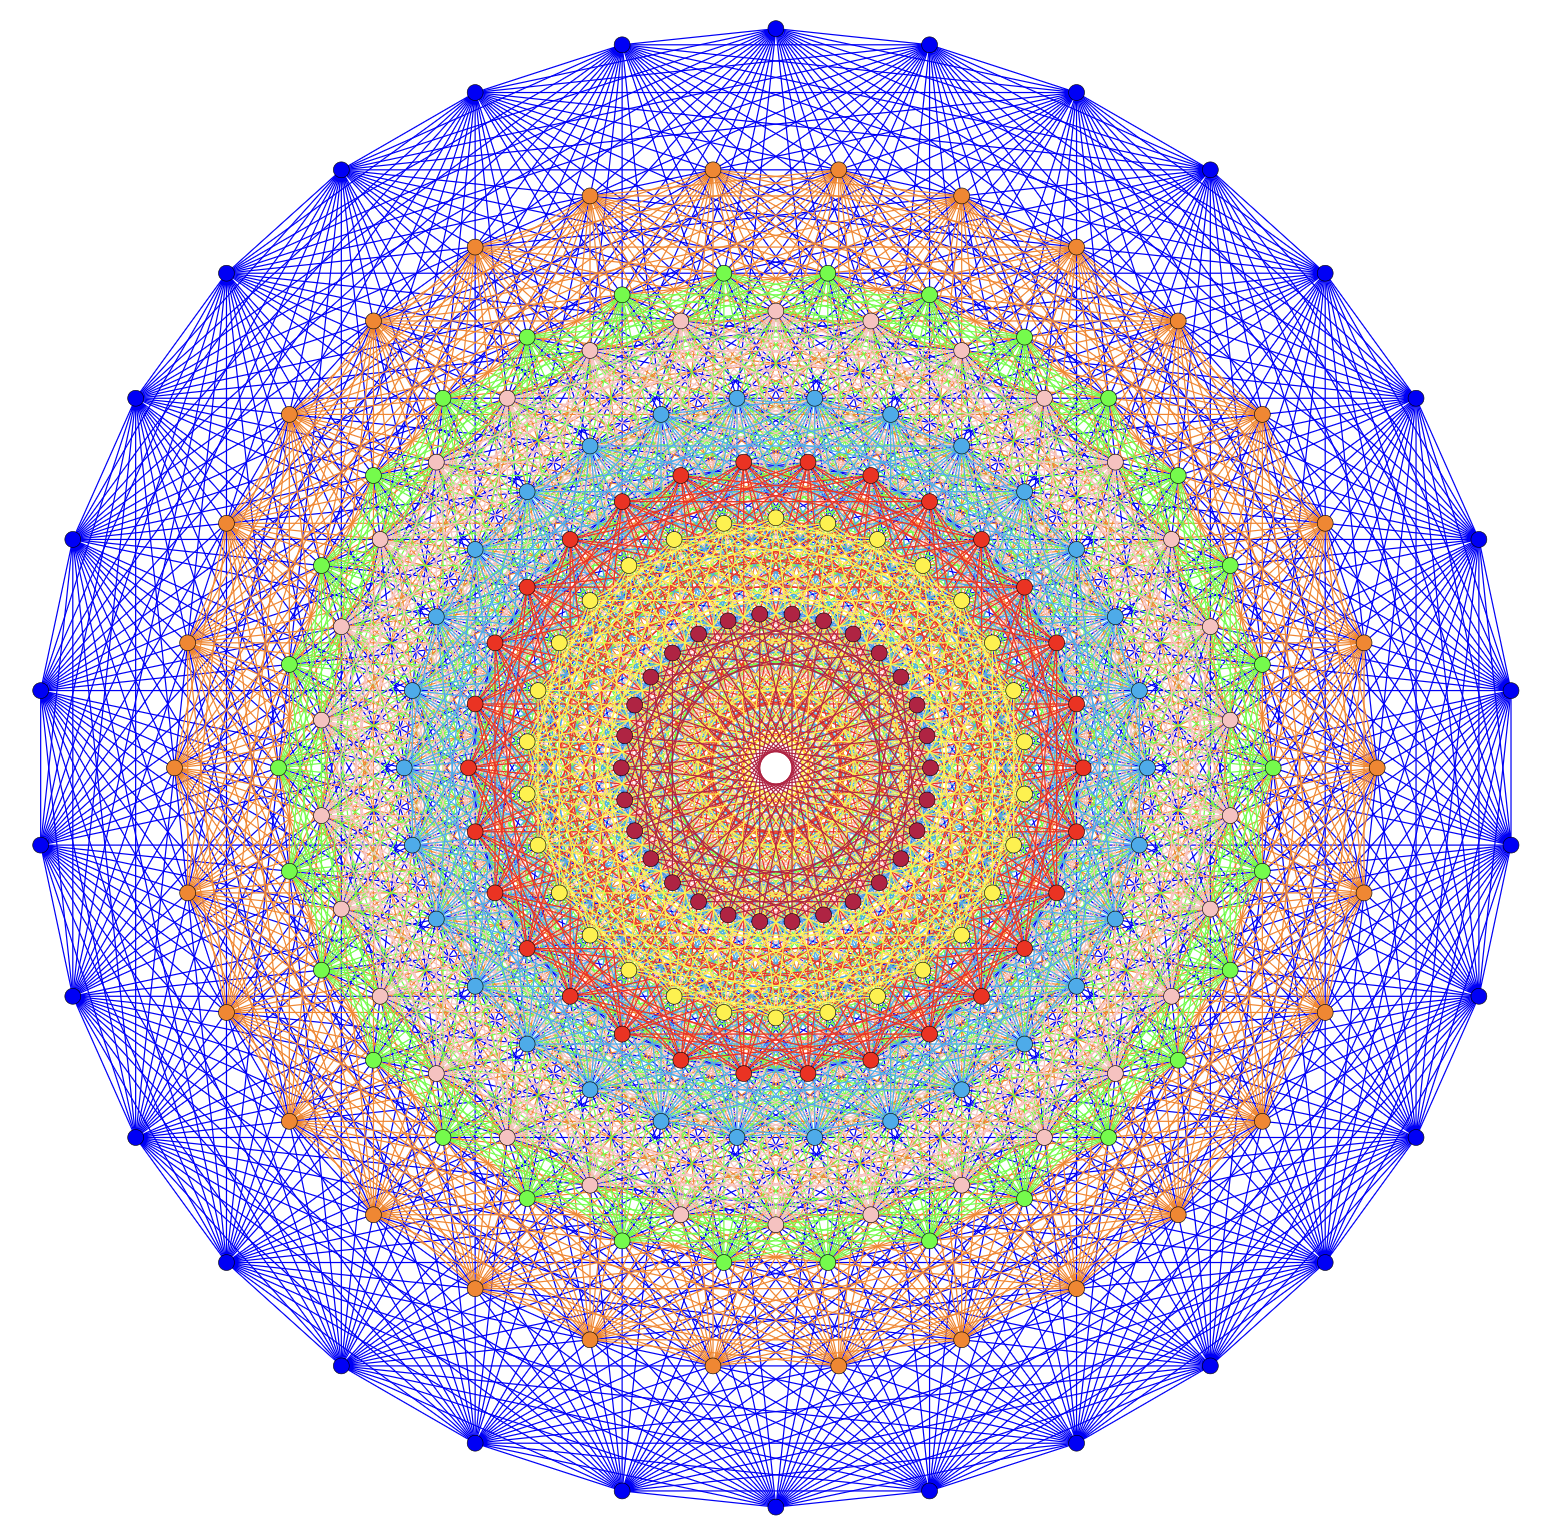
\includegraphics[width=0.98\linewidth]{Chapters/2_Dimension_8/Images/Gorbe_E8.png}
    \caption{The Coxeter projection of the $E_8$ root system. \cite{Gorbe_E8}}
    \label{Ch2:Fig:Gorbe_E8}
\end{wrapfigure}

It is quite remarkable that $E_8$ should show up when discussing sphere packings. At its core, $E_8$ is an irreducible root system. It shows up in the classification of important classes of objects like irreducible Coxeter groups, crystallographic Coxeter groups, and semi-simple Lie algebras over $\C$. $E_8$ is not a classical root system but an \textit{exceptional} root system, meaning that the geometric properties of its roots cannot be found in irreducible root systems in all dimensions.

The $E_8$ root system consists of $240$ vectors in $\R^8$ that are permuted by a certain finite subgroup of the $8$-dimensional orthogonal group. This group is sometimes referred to as the $E_8$ Coxeter group or as the Weyl group of the $E_8$ lattice. These roots can be divided into $8$ orbits, each of which corresponds to one of the `layers' of concentric circles in \Cref{Ch2:Fig:Gorbe_E8}. The dots in the figure correspond to projections of the roots onto a plane on which a specific type of element of the Coxeter group, known as a Coxeter element, acts as a rotation. This visualisation offers a convenient---and aesthetically pleasing---means of visualising this collection of $8$-dimensional vectors and appreciating some of its symmetry.

% From a motivational standpoint, this is quite important. So mention facts like distances between lattice points and things like that. Important for construction of magic function.

\sorry

\begin{boxtheorem}\label{Ch2:Thm:E8_Self_Dual}
    The dual lattice of the $E_8$ lattice is the $E_8$ lattice itself. That is, $\parenth{E_8}^* = E_8$ as free $\Z$-submodules of $\R^8$.
\end{boxtheorem}

This follows directly from the definitions of the dual lattice (\Cref{Ch2:Def:Dual_Lattice}) and the $E_8$ lattice (\sorry). This result will be useful later on, as it will give us an insight into the desired properties of the magic function.

\section{The Cohn-Elkies Linear Programming Bounds}\label{Ch2:Sec:CohnElkies}

Arguably, the result that most radically changed the sphere packing game was the linear programming bound constructed by Henry Cohn and Noam Elkies~\cite[Theorem 3.1]{CohnElkies}. The bound transforms the sphere packing problem from a geometric one to an analytic one. For all $d \in \N$, it posits the existence of a family of upper-bounds on the sphere packing constant $\Delta_d$, indexed by functions $f : \R^d \to \R$ that satisfy certain conditions.

The power of this result is that it offers a systematic approach to prove that a certain sphere packing $\Pa$ is optimal in $\R^d$. The optimality condition means that the density of $\Pa$ is equal to the sphere packing constant $\Delta_d$, which is equivalent to requiring that the density of $\Pa$ be greater than or equal to the density of any other packing in $\R^d$. The theorem proved by Cohn and Elkies tells us we can accomplish this by
\begin{enumerate}
    \item identifying a function $f : \R^d \to \R$ that satisfies the conditions of the theorem, giving an upper-bound for $\Delta_d$, and
    \item showing that the upper-bound indexed by $f$ is equal to the density of the packing $\Pa$.
\end{enumerate}
As simple as this sounds, it took close to fourteen years from the publication of Cohn and Elkies's paper for it to be used to concretely construct an optimal sphere packing. The real trick is to construct the right function $f$ to use in the process outlined above. We shall soon see the non-triviality of this task first-hand.

The original result~\cite[Theorem 3.1]{CohnElkies} is a bit different from the version that was chosen to be formalised. Firstly, the original result was stated for a very general class of functions known as \textit{admissible functions}. For our purposes, however, it suffices to look at Schwartz functions, which are not only admissible but also have useful properties that we will exploit later. We will remark, however, that at the time when Cohn and Elkies proposed their bound, it was not known that the solution to the sphere packing problem in dimensions $8$ and $24$ would only involve Schwartz functions. Furthermore, it might be possible that solutions in other dimensions would require the full generality of Cohn and Elkies's original result. Nevertheless, we will restrict our attention to Schwartz functions for the time being, not only because it is sufficient for our purposes but also because the theory of Schwartz functions has been developed quite substantially in \mathlib.

Another minor difference between the original result and the version we work with is that the original result was stated as an upper-bound on all \textit{centre densities} of sphere packings. The centre density of a sphere packing is merely a rescaling of its density by a factor of $\Volof{B_d\of{0, 1}}\inv$. Instead of encoding the information of the amount of sphere packing volume per unit volume of the ambient space, the centre density encodes the information of the number of centres of the sphere packing per unit volume of the ambient space. We sidestep these nuances by stating the result in terms of quantities we have defined.

\begin{boxtheorem}[Cohn and Elkies, 2003~{\cite[Theorem 3.1]{CohnElkies}}]\label{SP:Thm:CohnElkies} % Make sure to include the original version before this and then this adaptation
    If $f : \R^d \to \R$ is a Schwartz function satisfying the conditions
    \begin{enumerate}[label = \normalfont(CE\arabic*)]
        \item\label{SP:CE1} $f$ is not identically zero.
        \item\label{SP:CE2} For all $x \in \R^d$, if $\norm{x} \geq 1$ then $f(x) \leq 0$.
        \item\label{SP:CE3} For all $x \in \R^d$, $\hat{f}(x) \geq 0$.
    \end{enumerate}
    then we have the following bound on the sphere packing constant $\Delta_d$:
    \begin{align*}
        \Delta_d \leq \frac{f(0)}{\hat{f}(0)} \cdot \Volof{B_d\of{0, \frac{1}{2}}}
    \end{align*}
\end{boxtheorem}
\begin{proof}
    Let $f : \R^d \to \R$ be a Schwartz function satisfying the conditions~\ref{SP:CE1}-\ref{CE3}. By \Cref{Ch2:Prop:Periodic_Const_eq_Const}, it suffices to prove that
    \begin{align*}
        \Delta_d^{\text{periodic}} \leq \frac{f(0)}{\hat{f}(0)} \cdot \Volof{B_d\of{0, \frac{1}{2}}}
    \end{align*}

\end{proof}
\section{A Word on Modular Forms}
\label{Ch2:Sec:ModForms}